\chapter{How does the GA perform on a TSP of a larger scale?}


\section{Introduction} %Introduction might not be necessary
\par
Considering the characteristics of a Genetic Algorithm, one can assume that they are not the standard method to use on problems of such a small scale as the problem discussed in Chapter 2, since manual or traditional methods can give the solution as well. GAs hold their real value in problems of a larger scale. Here they are capable of giving a feasible solution, where most other methods fail to give one or are just highly inefficient. The constructed GA has proved itself capable of dealing with a simple TSP containing six cities, but how does it perform on a TSP of a larger scale? This chapter will discuss the answer to that question, explaining the obstacles encountered along the way.
\par
The details of the TSP, such as the number of cities and their locations, will be addressed in the next section of this chapter. Then in the third section, the first performance of the GA on this TSP will be discussed. Since the total of possible tours was relatively low for the simple TSP, discussed in the previous chapter, the GA was capable of finding the optimal tour in every run. In this larger TSP however, the number of tours is significantly larger, which meant that the GA did not find the optimal tour in every run. This problem is known as premature convergence and is the topic of the fourth section. In the last section of this chapter a possible method to prevent premature convergence is discussed.

\section{A TSP containing 26 cities} %Introducing the 26 cities TSP
For this expansion it was decided to extend the problem to 26 cities. To make the problem more realistic, these 26 cities were selected to be located throughout the Netherlands. 

\begin{table} [t]
\parbox{0.4\textwidth}{

	\begin{tabular}{l}
		1 Amersfoort\\ 
		2 Amsterdam\\
		3 Apeldoorn\\
		4 Arnhem\\
		5 Assen\\
		6 Breda\\
		7 Den Haag\\
		8 Den Helder\\
		9 Eindhoven\\
		10 Emmen\\
		11 Enschede\\
		12 Groningen\\
		13 Haarlem\\
		14 Heerenveen\\
		15 Heerlen\\
		16 ‘s-Hertogenbosch\\
		17 Leeuwarden\\
		18 Lelystad\\
		19 Maastricht\\
		20 Middelburg\\
		21 Nijmegen\\
		22 Rotterdam\\
		23 Tilburg\\
		24 Utrecht\\
		25 Venlo\\
		26 Zwolle
	\end{tabular}
	\label{26cities}
}
\qquad
	\begin{minipage}[c]{0.6\textwidth} 
		\centering
			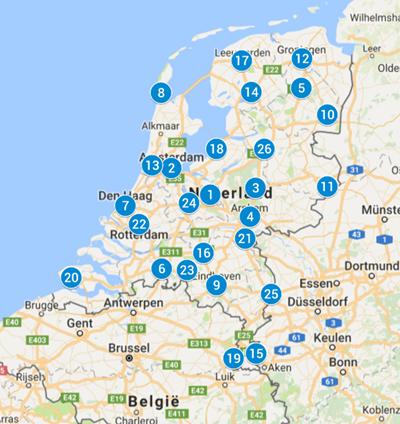
\includegraphics[width=1.2\textwidth, center]{26cities}
		\captionof{figure}{26 cities, marked on the map of the Netherlands\cite{Google}}
		\label{map1}
	\end{minipage}
\end{table}

\newpage
\par
The 26 cities are listed in alphabetical order together with a map of the Netherlands (figure \ref{map1}), that marks all of their locations. The objective is thus to find the shortest route that visits all of these cities and returns to the starting point afterwards. The total number of possible tours here is calculated by equation: %future reference needed
\[n = \frac{(26-1)!}{2} =  7.755605e+24\]
This number is significantly larger than the 60 possible tours for the simple TSP, discussed in chapter 2. This is then also the reason why most other methods fail to give a solution or are just inefficient. The manual methods and traditional methods, discussed in the previous chapter, are excellent examples. The Hungarian Algorithm already took 2 hours to perform on a TSP, containing only six cities and even though it did give the optimal solution in the end, it is highly inefficient to apply to this TSP because of the time it would take. In addition, this algorithm is a manual method, which makes it susceptible for human errors. The BIP also fails to give a solution, because the number of integer variables exceeds the limit of the Microsoft Excel linear solver. Even without this limit of variables, a BIP would take a long time to construct, considering all the possible subtours that would have to be added to the program as constraints in order to make sure that the resulting tour meets the criteria, set by the TSP. All of these subtours have to be excluded by manually adding these constraints, which makes the BIP timewise an inefficient method.Therefore it is necessary to turn to other methods, such as Genetic Algorithms. Even though they are not bound to give the optimal solution, they are at least capable of giving a suitable tour that meets the criteria, set by the TSP.



\section{The performance of the GA} %About the performance of the GA
\par
The first observation, when the GA was applied to the expanded TSP, was that the time for one run of the program had increased. Depending on the settings, such as the number of generations and the poolsize, the program now takes approximately a minute. Since one chromosome now consists of not 6, but 26 genes, it makes sense that the time for one run increased. One minute is still a relatively short amount of time to find a solution. Besides the short time, another benefit is that the GA did not need reconstructing in order to be applied to this expanded TSP. Because of the way the basic structure was programmed, this GA can be applied to any TSP, that sparks your interest given that you provide the necessary data, which consists of the number of cities and their distances to each other. For other methods, like the Hungarian Algorithm or the BIP, this does not hold. 

\begin{wrapfigure}{r}{0.5\textwidth}
	\vspace{-1cm}
	\begin{center}
		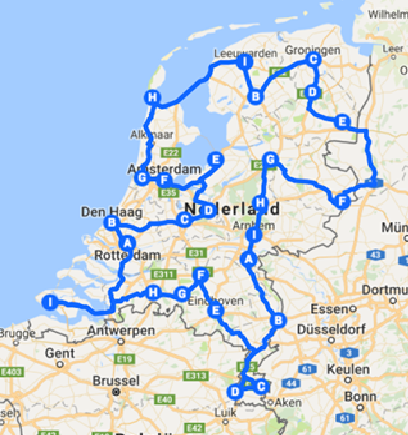
\includegraphics[width=0.48\textwidth]{1406tour}
	\end{center}	
	\captionof{figure}{The tour with a total distance of 1406 kilometers \cite{Google}}
	\label{1406tour}
\end{wrapfigure}

The next observation was that, while the GA still converged to a solution in every run, these solutions differed from each other. They did not show the same tour nor did they share the same total distance. The solutions seemed to span a reach of approximately 100 kilometers, the lowest solution having a total distance of 1406 kilometer. The tour, belonging to this solution of 1406 kilometers, is shown in the figure below. During the analysis of the constructed GA, the program never gave a tour with a lower distance than this 1406 kilometers. We therefore believe this solution could well be the optimal tour however, due to the large amount of possible tours, this cannot be said with full certainty. 

\clearpage
\par
In order to find out why the GA gave multiple solutions, a new variable was introduced to the program. This variable, named LEETchanges, counts the number of times the best chromosome in the pool, meaning the chromosome with the lowest total distance, is changed. Additionally the program also outputs when the last LEETchange has occurred. The conclusion, drawn from analyzing this new variable, was that the program reached convergence too fast. The last change of the best solution in the pool nearly always occurred in the first quarter of the number of generations. For example, if the number of generations was set to a 1000 then in generation 200 the best solution was last changed. This means that in generation 201 up until 1000 the best solution always remained the same tour. However, this solution was not necessarily the tour with the lowest total distance, since for one run the solution came out with a total distance of 1547 kilometers and for another run the total distance was 1422 kilometers. Therefore the program does not converge to the optimal solution every time. The program suffered from premature convergence, which is the topic of the next section. 

\section{Premature Convergence}

\par

\begin{wrapfigure}{r}{0.5\textwidth}
			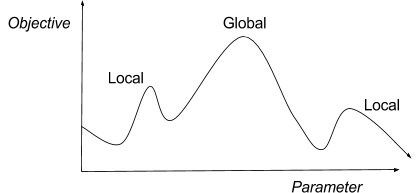
\includegraphics[trim = {0 0 5mm 0}, clip, scale = 0.5]{PrematureConvergence}
	\captionof{figure}{Visualization of a one-dimensional problem}
	\label{PrematureConvergence}
\end{wrapfigure}

Premature convergence is when the GA converges too early, to a local optimum.
It can be visualized by figure \ref{PrematureConvergence}. This graph, representing a one-dimensional problem, shows multiple peaks, several being local optima and one being the global optimum. When the program converges to a local optimum, i is unlikely to get past that local optimum to a better solution. Due to the concept of “survival of the fittest”, the best solution in the pool has the highest chance of being selected as a parent. If that best solution is in the neighborhood of a local optimum, then the majority of its children will also be in the neighborhood of that local optimum. In the following crossovers, a pool is generated with more and more chromosomes that are clustered around this local optimum. In other words, the selected parents cannot create children that are superior than they are themselves. Therefore the GA will not get past the local optimum during crossover. Moreover, the population loses its diversity as the program goes through the set number of generations, this is believed to be the main reason for the occurrence of premature convergence \cite{Premconvergence}\cite{Popdiv}\cite{Congress}.

\par
To obtain a chromosome, which is better than the current best solution in the pool, mutation is the only hope. As already mentioned by equation, there are 7.755605e+24 possible tours if duplicates and mirrored solutions are excluded. The GA however, does not necessarily exclude duplicated and mirrored tours, therefore the number of tours that the GA accounts for is: 26! = 4.0329146e+26. The size of this number makes the chance of randomly mutating a tour to a better solution than a local optimum very small. Even changing the rate of mutation, thus making the mutation more frequent and aggressive, will not prevent premature convergence. It is therefore also a frequent problem, encountered when applying GAs to optimization problems. 

\section{Incest Prevention}

\par
There are different methods of dealing with premature convergence. H. Pandey, A. Chaudhary and D. Mehrotra discuss 24 methods in their article \textit{A comparative review of approaches to prevent premature convergence in GA}\cite{Premconvergence}. In this section one of those methods will be discussed, namely incest prevention. Incest prevention is preventing two identical parents from breeding. During a crossover where two identical solutions are selected as the parents, two children will be created that are both identical to their parents and to each other. By constantly breeding with two identical parents, the generated pool quickly loses its diversity, which is the main cause of premature convergence. Which part of the parents is selected does not influence the outcome of such a crossover. Take for example a crossover between two identical parents, both containig six indices:
\newline
\textit{Parent 1} =  0 1 2 3 4 5 
\newline
\textit{Parent 2} =  0 1 2 3 4 5 
\newline
In the first crossover a part of the first parent is selected and the remaining indices are provided in the order they appear in the second parent. This could happen in the following way: 
\newline
\textit{Parent 1}: - 1 2 3 - -                 
\newline
\textit{Parent 2}: 0 - - - 4 5
\newline
This leads to \textit{Child 1}: 0 1 2 3 4 5

\par
From this first child, it can be easily seen that the second child will also be identical to the parents and its sibling. However, this only happens, when both of the parents are completely identical, meaning that both their tour and starting location have to be the same. For example a crossover between the parents, depicted below, does not necessarily lead to a child that is identical to the parents, even though they share the same tour:
\newline
\textit{Parent 1} =  0 1 2 3 4 5 
\textit{Parent 2} =  2 3 4 5 0 1 
In the first crossover, where a subset from the first parent is selected and the remaining parts of the chromosome are given by the second parent, this could happen:
 \newline
Parent 1: - 1 2 3 - -                 
\newline
Parent 2: - - 4 5 0 -
\newline
This leads to \textit{Child 1}: 4 1 2 3 5 0
 \newline
Even though both parents contained the same tour, their child does not share it. Incest prevention therefore focuses on only eliminating crossovers between two identical parents. Incest prevention therefore focuses on only eliminating crossovers between two identical parents.

\par
In order to implement incest prevention in the GA, an adjusted form of tournament selection was used. The first parent is still selected by means of probability based on its fitness. However, the second parent is now selected by a tournament of a set number of chromosomes. The winner of the tournament is the chromosome that is most different to the already selected first parent. If all candidates in the tournament are identical to the first parent, the program will dismiss the tournament and start a new one. This process goes on until a different chromosome is found. 

\par
The result of implementing this into the GA was that it increased the time for one run of the program. With the same settings, the time about doubled. This large increase can only be explained by the tournaments, since they were the only addition to the GA. This gives a helpful insight in the GA, since it apparently has to run a high amount of tournaments. This means that in most of the tournaments candidates are selected that are identical to the already determined first parent. Although the incest prevention itself works, the GA still converges to local optima. The incest prevention therefore did not prevent premature convergence and since it causes a large increase in time, it is not recommended to use within this GA and has not been used in the next section. 

\section{Further expanding the TSP}
\par
The GA is more than capable of dealing with a further expansion of the TSP, since when it contained 26 cities it gave solutions in approximately a minute. Therefore in this section, the GA will be applied to a TSP containing 50 cities, still all located throughout the Netherlands. Here the number of possible tours is the extremely high value of:
\[n = \frac{(26-1)!}{2} = 3.0414093e+62\]
To put this number in perspective, there are more possible tours for this problem than there are atoms in the earth. Moreover, the GA itself accounts for even more tours, namely $50! = 3.0414093e+64$. Considering that traditional methods, like the Hungarian Algorithm or the BIP, were concluded to be unsuitable for the TSP consisting of 26 cities, they can be concluded even more unsuitable for this TSP, containing 50 cities.

\begin{wrapfigure}{r}{0.43\textwidth}
	\vspace{-0.4cm}
	\centering
		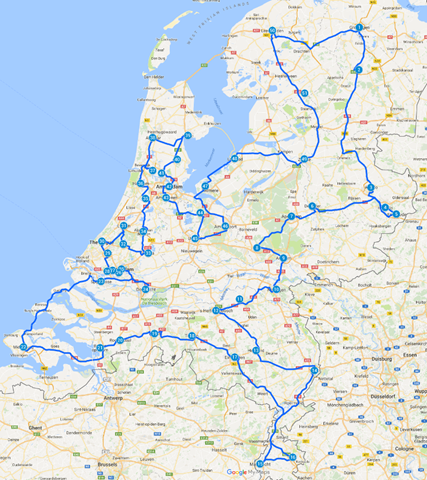
\includegraphics[width=0.41\textwidth]{1623tour}	
	\captionof{figure}{The tour of 1623 kilometers \cite{Google}}
	\label{1623tour}
\end{wrapfigure}

\par
The first observation to note is again an increase in time. Where the GA took 1 minute to complete the set number of generations for a TSP of 26 cities, the GA now takes 6 minutes with the same settings. Yet 6 minutes is a very short amount of time if one considers the number of possibilities, given in the previous paragraph. The GA still suffers from premature convergence and in order to work around that issue, the GA was set to run 600 times, saving the final solutions to an external file. Out of all these runs, the best solution, given by the GA, was a tour of 1623 kilometers. This tour is shown in figure \ref{1623tour}. Because of the large number of possible tours, it cannot be said with certainty that this tour is in fact the global optimum 


\section{Conclusions}
\par
This chapter has dealt with the question: How does the GA perform on a problem of larger scale? This problem contained 26 cities located throughout the Netherlands. The GA was still capable of converging to a solution however, these solutions are not necessarily the optimal tour. In other words, the program suffered from premature convergence. One method was examined to prevent this from happening, but without success. It is also outside of the range of this research to prevent the premature convergence. While it is true that the GA will sometimes give a tour that is not the global optimum, the chance of selecting a better tour by random choice is very very low due to the sheer amount of possible tours. 

